\documentclass[a4paper,12pt,openany]{report}

\usepackage{titling}
\usepackage[margin=0.75in,headsep=0.5in,footskip=0.5in]{geometry}
\usepackage{graphicx}
\usepackage{float}

\setlength{\parindent}{12pt}

\newcommand{\subtitle}[1]{
	\posttitle{
		\par\end{center}
		\begin{center}\large#1\end{center}
		\vskip0.5em
	}
}

\newcommand{\coverphoto}[2]{
	\postdate{
		\par\end{center}
		\begin{center}
			\includegraphics[width=15cm]{#1}
		\end{center}
	}
}



% document

\begin{document}

% Title Page

\title{CITS3001 Algorithms and Artificial Intelligence}
\subtitle{Threes Bot - Artificial Intelligence Project}
\author{Mitchell Pomery (21130887)\\
Kieran Hannigan (21151118)}
\coverphoto{images/constructive}{XKCD 810}
\maketitle

\clearpage

% Introduction
\section*{Introduction}

% What is Threes

\paragraph \indent
Threes\cite{threes} is a simple mobile game where you are given a four by four grid occupied by tiles.
The aim is to merge tiles until the board is full and no more merges are possible, or until there are no tiles left to be added to the board.
Each move (left, right, up or down) moves each tile one space on the grid if it is free, or merges it with the tile it moves into if conditions are met.
You are only able to merge a one tile with a two tile, and any other tile can be merged with another of the same value.
We were tasked with the creation of an artificial intelligence to play the game Threes, the goal being to get the highest score possible given a board and a list of upcoming tiles.

\begin{figure}[h!]
	\centering 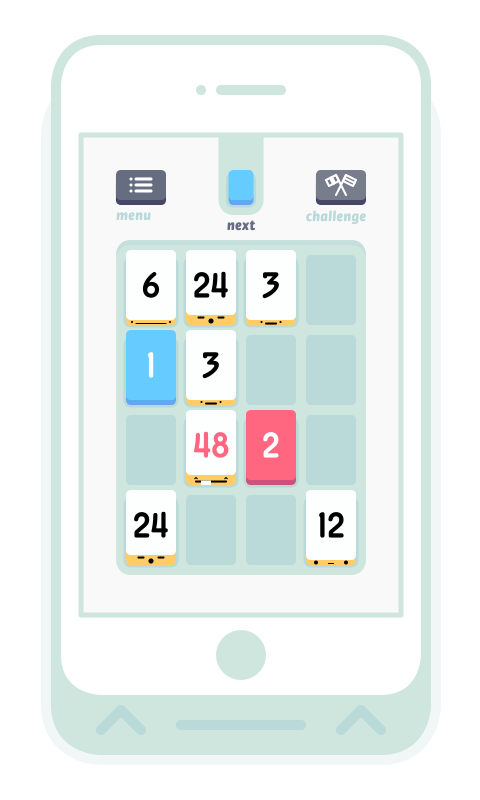
\includegraphics[scale=0.2]{images/THREES_phonepromo}
	\caption{Threes Mobile Game Promotional Image}
\end{figure}

% What Exactly Are We doing

\paragraph \indent
We were required to investigate algorithms and implementations to create an artificial intelligence, or bot, to play Threes with the intent of getting as high a score as possible.
The specifications for the bot stated three main points that were considered during the design and implementation.
\begin{enumerate}
	\item All upcoming tiles are known
	\item Tile placement is deterministic
	\item Inputs will be large
\end{enumerate}

\paragraph \indent
Knowing all upcoming tiles, and by being able to determine the location they will be placed means that at each node, there are only up to 4 different moves that can occur.
Large input data sets remove the ability to search all possible combinations of moves, meaning that either a search depth or a maximum search time needs to be implemented.


% Design Choices

\section*{Design Choices}

% Language Choice
\subsection*{Programming Language}
\paragraph \indent
Python was chosen as the initial implementation language due to the ability to rapidly prototype different algorithms and data structures.
Its automatic handling of memory is convenient, and its syntax makes it easy to read and intuit - valuable attributes when co-developing an artificial intelligence.
Subsequently, we began a rewrite of the agent to C.
This allowed us to evaluate the strength and weaknesses of each language - an analysis which would have to be conducted if the code was to be hard optimized for production.
Whilst python is conducive to comprehensible code, C outperforms any high level language when it comes to space and speed requirements.
We reprogrammed the board mechanics, priority queue, and greedy algorithm in C for evaluation.
The result was verbose, but faster.

% AI Considerations

\subsection*{AI Considerations}
\paragraph \indent
To make our artificial intelligence achieve the highest score, we need to score each board layout against several criteria.
These criteria are essentially questions that can be asked to determine how good the board is, and therefore can be used to rank several boards.
The boards score was the initial measurement used to rank different board combinations, due to the fact we are aiming for the maximum board score.
The number of empty locations on the board is a useful measurement that we considered.
Less tiles on the board means that we can add more tiles, and hence more points, without merging tiles to achieve a higher score.

\paragraph \indent
The location of the high number tiles is important in a boards configuration.
Having the high number tiles in the central four squares on a board means that they are stopping the lower tiles from residing next to each other.
Smoothness of the board was considered after reading a Stack Overflow thread on 2048 artificial intelligence algorithms\cite{2048so}.
Smooth board layouts mean that high numbered tiles are clustered in one corner.
These two criteria are similar as both relate to the layout of the board, so they are be converted into a single measure. The highest performing heuristic that we could device incorporated a factor of the score, the emptiness of the board, the gradient of lines (rows or columns that increase at every step are rewarded), and the edge-heaviness of the board (higher tiles on the outside ring give better results).

% Algorithms

\section*{Algorithms}

\subsection*{Making Moves}
\paragraph \indent
There are two ways the moves can be implemented in the bot, either each possible move separately, or by rotating the board and treating all moves as the one direction.
In our python implementation we employ the latter of the two algorithms, as it allows us to reduce the amount of code written. However rotating a sixteen by sixteen board can take several operations, so to avoid this, instead of rotating the board, we rotate the co-ordinates.
In our C experiment, we move the board using loops and array operations.
We also experimented with large integer bitboards.
A 64 bit bitboard allows for each tile to be encoded in a 4 bit nybble.
Unfortunately this means a maximum tile size of 12288 which we predicted would be readily achievable by a fully optimized algorithm. Bitboards are optimal because they provide the CPU with a memory unit that it can make extremely efficient shift and addition operations on (holding it in a single register).
Unfortunately this advantage is largely lost when multiple bitboards or 128 bit bitboards are used -- as would be required for the tile size -- especially on machines with 32 bit registers.
We opted to use more portable code here.

\subsection*{Naive}
\paragraph \indent
Initially a naive algorithm was implemented to play Threes one move at a time.
It would look at the four possible moves for the current board configuration (left, right, up and down), and execute the one that gives it the highest score.
The naive algorithm is useful as an initial heuristic later in the A* implementation.
In the C port, we provided a simple ``count the zeros'' heuristic to the naive algorithm.
We found that by minimizing the tiles on the board instead of chasing high tiles, the algorithm produces a better final result.

\subsection*{Minimax}
\paragraph \indent
Both minimax and expectiminimax implementations were investigated due to the similarities between Threes and 2048, and the already existing 2048 AI by Matt Overlan\cite{2048ai}.
A major difference between 2048 and Threes is that in 2048 the next tile is placed randomly, while Threes as specified by the project outline, the location of the next tile will be placed in the lexicographical lowest location.
This difference means that the Threes bot does not end up playing against anything -- it becomes a deterministic problem as opposed to a stochastic one -- and so minimax is not a relevant algorithm.

\subsection*{A Star}
\paragraph \indent
A*, by definition, finds the least-cost path from the initial state to a goal state providing that its algorithms are correct and admissible.
It is easy to devise monotonic heuristics for Threes, making A* particularly promising.
The goal state in a game of Threes is the highest scoring full board, meaning that the algorithm needs to avoid filling the board for as long as possible.
Multiple iterations of A* algorithms were implimented to glean a measure of the effectiveness of each heuristic.

% Test Data

\section*{Test Data}
\paragraph \indent
Test data was generated using a modified version of \texttt{createTestData.py} by Lyndon While\cite{testdatagenerator}. 
It was modified to create multiple ouput files with 1000 upcoming tiles in one run of the program.
\texttt{test.py} would then be used to load the input files and run them through the written algorithms, outputting the data in CSV form for analysis.

\paragraph \indent
Testing was done over three algorithms, the naive implimentation, a naive A* implimentation and our final A* implimentation.
We found that the naive algorithm would quickly fill up all the available space on the board whereas the naive A* would avoid filling the board for as long as possible.
The final A* implimentation we created as depth limited and had similar final scores as the naive A* implimentation but took half the time.

\begin{center}
\begin{tabular}{|  l | r | r |}
	\hline
		\textbf{Algorithm} & \textbf{Average Time(ms)} & \textbf{Average Score} \\ \hline
		Naive & 18 & 305 \\ \hline
		Naive A* & 31951 & 7665 \\ \hline
		Final A* & 17670 & 6731 \\
	\hline
\end{tabular}
\end{center}

% bibliography

\begin{thebibliography}{20} 
	\bibitem{threes} THREES - A tiny puzzle that grows on you. 2014. [ONLINE] Available at: http://asherv.com/threes/. [Accessed 28 May 2014].
	\bibitem{2048ai} 2048. 2014. [ONLINE] Available at: http://ov3y.github.io/2048-AI/. [Accessed 28 May 2014].
	\bibitem{2048so} logic - What is the optimal algorithm for the game, 2048? - Stack Overflow. 2014. [ONLINE] Available at: http://stackoverflow.com/questions/22342854/what-is-the-optimal-algorithm-for-the-game-2048. [Accessed 29 May 2014].
	\bibitem{testdatagenerator} createThreesFiles.py. 2014. [ONLINE] Available at:\\
		http://undergraduate.csse.uwa.edu.au/units/CITS3001/project/createThreesFiles.py. [Accessed 30 May 2014].
\end{thebibliography} 


\end{document}
